\section{SCLDPC Lattices for Interference Channel}
%%---------------------------------------------------------------------------------------------------------------
\begin{frame}\frametitle{Lattices and Lattice Codes}
	New perspectives for dealing with interference:
      \begin{itemize}
     		\item Interference alignment - Sridharan, Jafarian, Vishwanath and Jafar
			\item Compute-and-forward - Nazer \& Gastpar
			\item Physical layer network coding - Wilson et al, Nam et al
      \end{itemize}

\begin{block}{}
		\begin{itemize}
			\item Above schemes are all based on good lattice codes.
			\item	\textit{Poltyrev-}good lattices are at the core of such lattice coding schemes
		\end{itemize}
\end{block}
\end{frame}

%%---------------------------------------------------------------------------------------------------------------
%\begin{Interference channel: Lattice coding}
\begin{frame}\frametitle{Symmetric Interference Channel}
	\begin{figure}
		\centering
		\only<1->{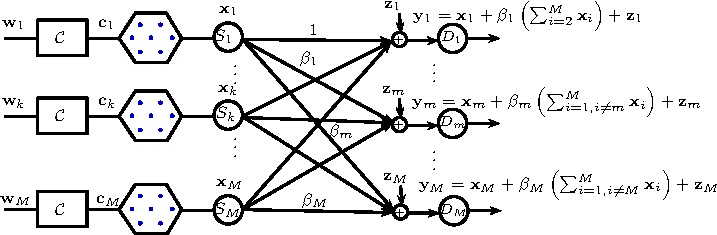
\includegraphics[width=4in]{\figpath/IC_model_ISIT}}
	\end{figure}
\end{frame}  

%%---------------------------------------------------------------------------------------------------------------
\begin{frame}\frametitle{Main Result}
	\begin{block}{Codes over $\mathbb{F}_{2}$ and BP decoding suffice}
			\vspace{1em}
		\begin{itemize}
			\item Recall Forney et al's result - based on nested random binary linear codes
			\item Propose capacity-achieving nested SC LDPC ensemble
			\item Construct lattices using Construction-D, based on the above ensemble
			\item Show existence of sequence of lattices that are \textit{Poltyrev}-good under BP 
		\end{itemize}			
	\end{block}
\pause
\vspace{2em}
   \begin{itemize}
	        \item Apply proposed lattice codes with hypercube shaping for the {\blue Symmetric Interference Channel}
    \end{itemize}
\end{frame}

\begin{frame}
   \begin{itemize}
	        \item Apply proposed lattice codes with hypercube shaping for the {\blue Symmetric Interference Channel}
    \end{itemize}
    \centering
   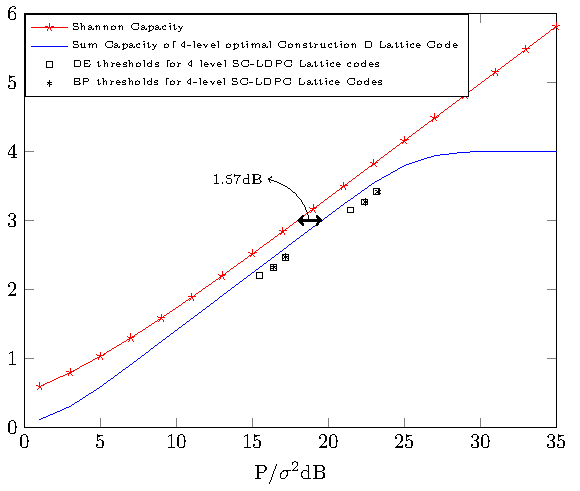
\includegraphics[width=2.75in]{\figpath/ShapingLoss_Final_CTW}
\end{frame}

%%---------------------------------------------------------------------------------------------------------------
%\begin{frame}\frametitle{Achievable Information Rates}
%    \begin{figure}
%        \begin{center}
%
%        \end{center}
%    \end{figure}
%\end{frame}